	En este capítulo mostramos los resultados del presente trabajo, comparamos los resultados de la ejecución de 5 modelos, los tiempos de ejecución y 
		comparamos los resultados obtenidos. Los modelos ejecutados tanto los originales, en PowerDEVS, y los modelos transformados en 
		$\mu$-Modelilca se encuentran en \url{https://github.com/lucciano/pd2mo/tree/master/doc/tesina/src}

\section{Comparación de performance}
	A continuación por cada uno de los modelos se muestra su modelo en PowerDEVS seguido de una gráfica de valores en tiempo de las simulaciones 
	(provista por ambas herramientas en GNUPlot), 
	a la izquierda se muestra el resultado en PowerDEVS y a la derecha los de QSS-Solver convertidos por la herramienta desarrollada.

\todo[inline]{Tratá de poner caption a todas las figuras y mencionarlas en el texto. En la figura tanto vemos el resultado de....} 
\todo[inline]{Lo mismo para las tablas!}

\section{Ecuaciones Lotka-Volterra}

\todo[inline]{Menciona que este es el sistema visto en el cap 2 y pasalo como primer ejemplo ya que es el más simple}
	El sistema de ecuaciones Lotka-Volterra, es un sistema de ecuaciones diferenciales de primer orden, no lineales, utilizadas para describir dinámicas de sistemas biológicos en el cual dos especies interactúan, una como presa y otra como depredador, se definen como:

\begin{align*}
\frac{dx}{dt} & = x(\alpha - \beta y)\\
\frac{dy}{dt} & =y(\gamma - \delta  x)
\end{align*}

donde:
\begin{itemize}
	\item y es el número de algún predador (por ejemplo, un lobo);
    \item x es el número de sus presas (por ejemplo, conejos);
    \item t representa el tiempo; y
    \item $\alpha$, $\beta$, $\gamma$, $\delta$ son parámetros que representan las interacciones de las dos especies.
\end{itemize}

	Este sistema es representado por el modelo siguiente:

\begin{figure}[H]
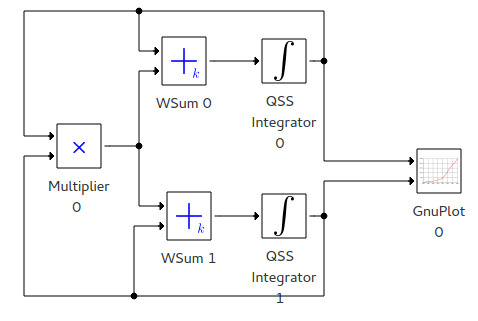
\includegraphics[width=0.75\linewidth]{lotka_voltera_pwd}
\caption{Modelo PowerDEVS del Sistema Lotka Volterra}
\label{model:lotka_voltera}
\end{figure}

\begin{figure}[H]
\centering
Resultados de la simulación \\
\begin{minipage}{0.5\textwidth}
\centering
 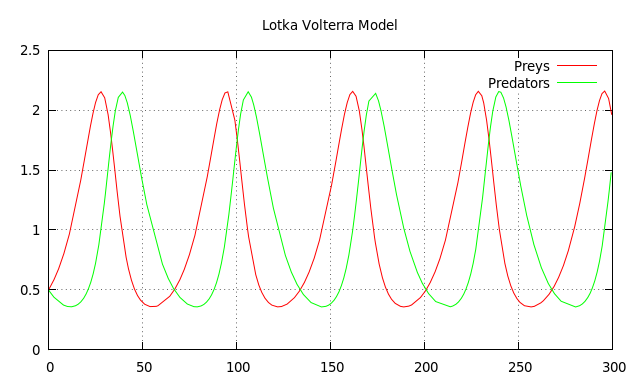
\includegraphics[width=\linewidth]{lotka_voltera-pd}
\caption{PowerDEVS}
\label{graph:lotka_voltera-pd}
\end{minipage}\hfill
\begin{minipage}{0.5\textwidth}
\centering
 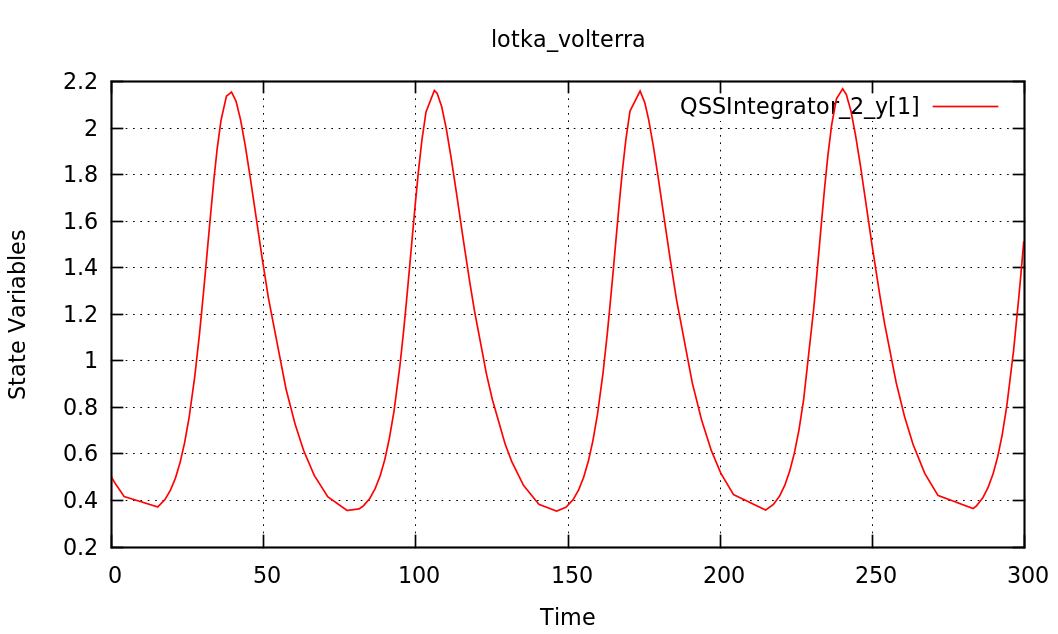
\includegraphics[width=\linewidth]{lotka_voltera-qss}
\caption{QSS-Solver}
\label{graph:lotka_voltera-qss}
\end{minipage}
\end{figure}



\section{Líneas de Transmisión}
	El siguiente sistema de ecuaciones representan un modelo a parámetros concentrados de una línea de transmisión formada por $N$ secciones de circuitos LC:

\todo[inline]{Usá la notación $\frac{d v}{d t}$ como en el cap 2}

\todo[inline]{Ojo que esa ecuación vale para j=2..N-1 para los bordes hay otras dos eq}
\begin{equation*}
\begin{split}
\dot{v}_{j} &= \frac{i_{j} - i_{j+1}}{C} \\
\dot{i}_{j} &= \frac{v_{j-1} - v_{j}}{L} \\	
\end{split}
\end{equation*}

para $j = 2 \dots N-1$

Consideramos también un pulso de entrada:
\begin{equation}
v_0(t) = \left\{ 
  \begin{array}{l l}
    1 \text{ si } t < 1 \\
    0 \text{ en caso contrario }
  \end{array} \right.
\end{equation}

\begin{figure}
 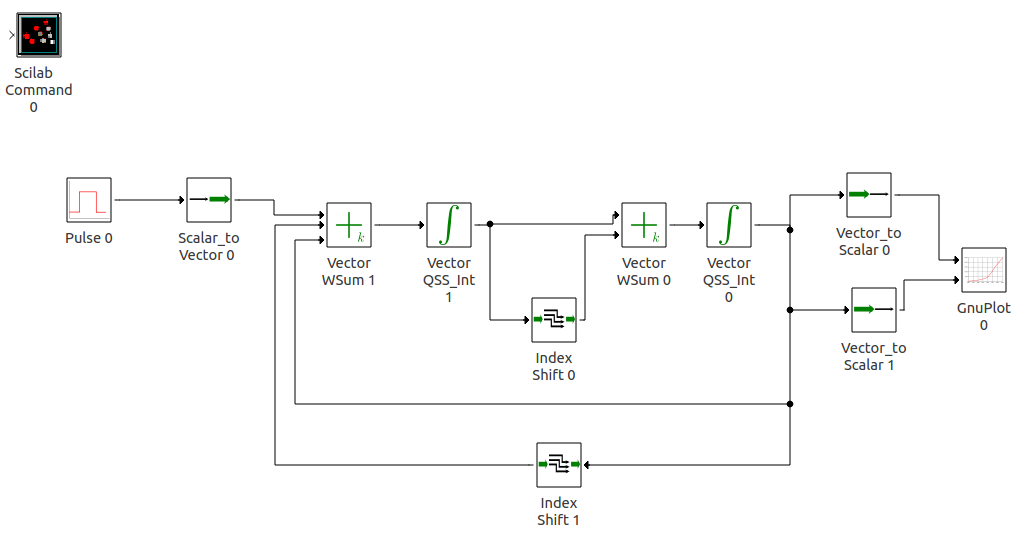
\includegraphics[width=0.75\linewidth]{lclines}
\label{model:lclines}
\caption{Modelo PowerDEVS de Líneas de Transmisión}
\end{figure}

\begin{figure}[H]
\centerfloat
\begin{minipage}{0.5\textwidth}
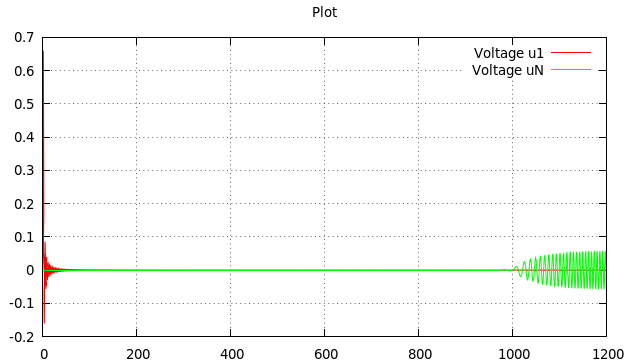
\includegraphics[width=\linewidth]{lcline-pd}
\label{graph:lclines-pd}
\caption{PowerDEVS}
\end{minipage}\hfill
\begin{minipage}{0.5\textwidth}
 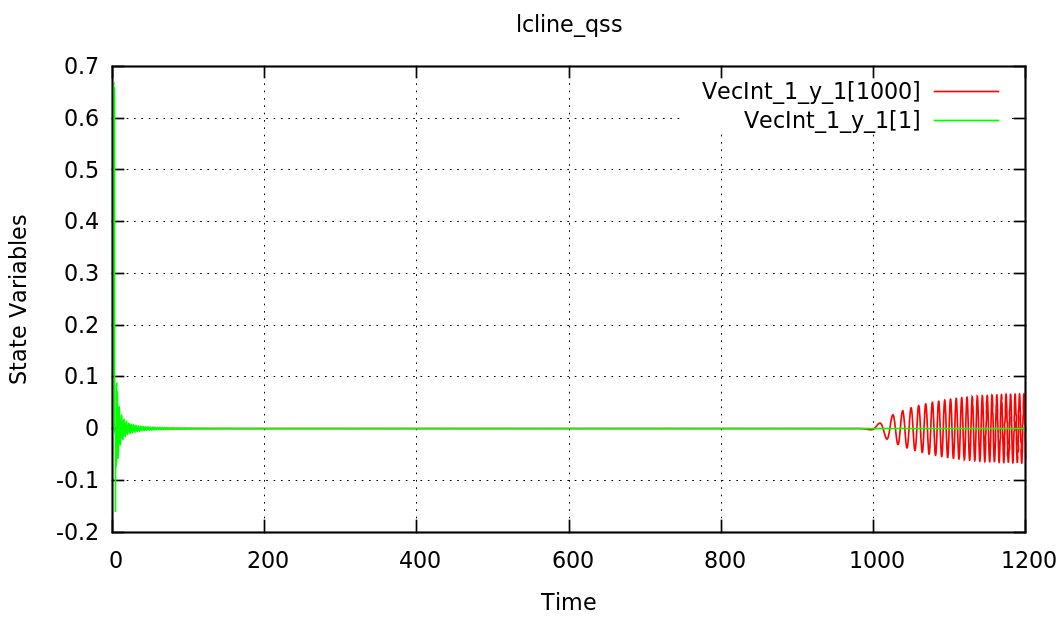
\includegraphics[width=\linewidth]{lcline-qss}
\label{graph:lclines-qss}
\caption{QSS-Solver}
\end{minipage}
\end{figure}

\section{Inversores Lógicos}
	El siguiente modelo representa una cadena de $m$ inversores lógicos, 

\todo[inline]{Usá la notación $\frac{d v}{d t}$ como en el cap 2}
\begin{align*}
\dot{\omega}_1 & = U_{op} - \omega_1(t) - \Upsilon g (u_{in}(t), \omega_{1} (t))    \\
\dot{\omega}_j & = U_{op} - \omega_j(t) - \Upsilon g (\omega_{j-1}(t), \omega_{j} (t)) \textrm{ donde $j = 2, 3, .., m$}
\end{align*}


\begin{figure}[H]
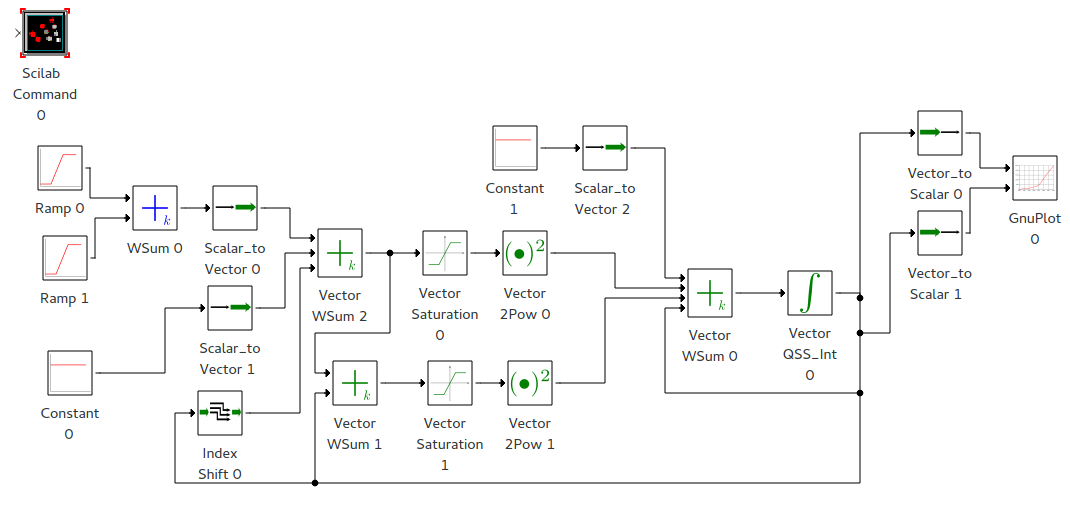
\includegraphics[width=0.75\linewidth]{inverters}
\label{model:inverters}
\caption{Modelo PowerDEVS de Inversores Lógicos}
\end{figure}

\begin{figure}[H]
\begin{minipage}{0.5\textwidth}
 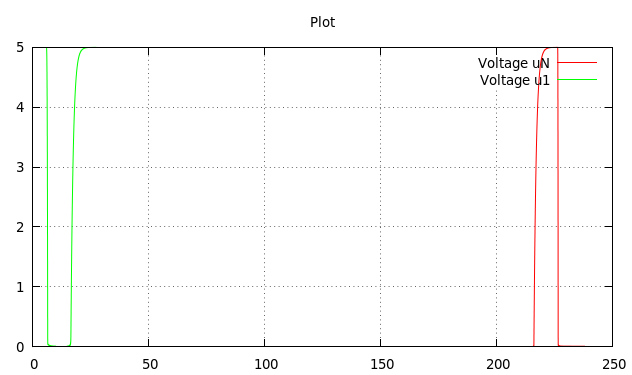
\includegraphics[width=\linewidth]{inversers-pd}
\label{graph:inverters-pd}
\caption{PowerDEVS}
\end{minipage}\hfill
\begin{minipage}{0.5\textwidth}
 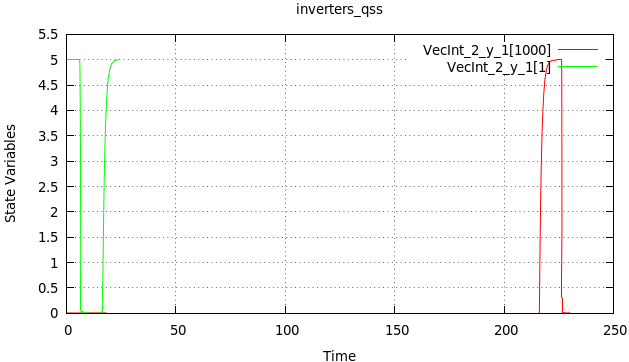
\includegraphics[width=\linewidth]{inversers-qss}
\label{graph:inverters-qss}
\caption{QSS-Solver}
\end{minipage}
\end{figure}

\section{Advection-Diffusion-Reaction}
	El modelo de equaciones Advection-diffusion-reaction (ADR) provee las bases para describir fenomenos de tranferencias de calor y masa, donde la cantidad de interes $u(x,t)$ puede ser temeratura en la conducción de calor o concentración de una sustancia química.

La ecuación 
\begin{equation*}
\frac{du(x,t)}{dt} + a \frac{du(x,t)}{dx} = d\frac{d^2u(x,t}{d^2x} + r(u(x,t)^2 - u(x,t)^3)
\end{equation*}
corresponde al modelo ADR, donde $a$,$d$ y $r$ son parametros expresando coeficientes de advección, difusión y reactión

\begin{figure}[H]
 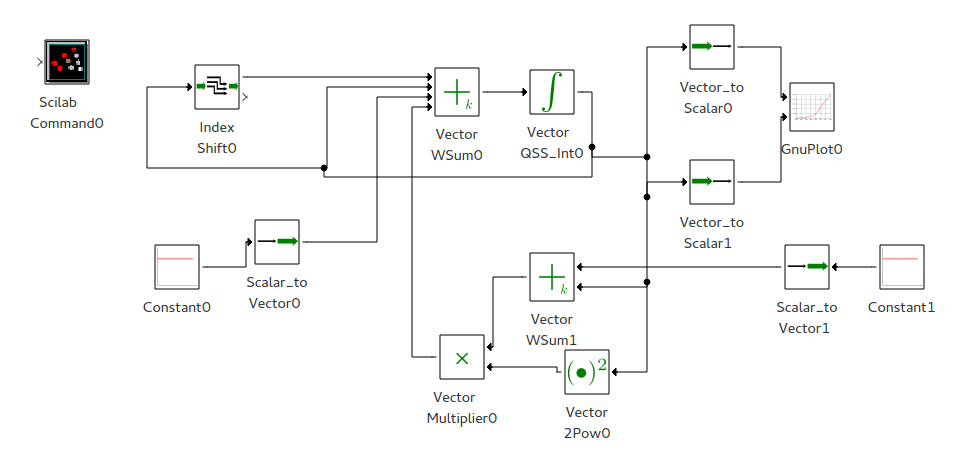
\includegraphics[width=0.75\linewidth]{adr-pwd}
\label{model:adr}
\caption{Modelo PowerDEVS ADR}
\end{figure}

\begin{figure}[H]
\begin{minipage}{0.5\textwidth}
 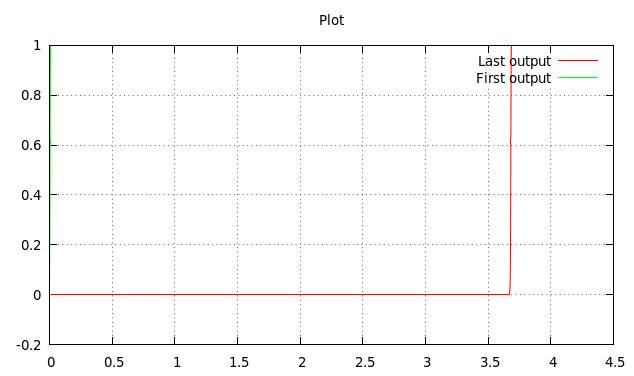
\includegraphics[width=\linewidth]{adr-pd}
\label{graph:adr-pd}
\caption{PowerDEVS}
\end{minipage}\hfill
\begin{minipage}{0.5\textwidth}
 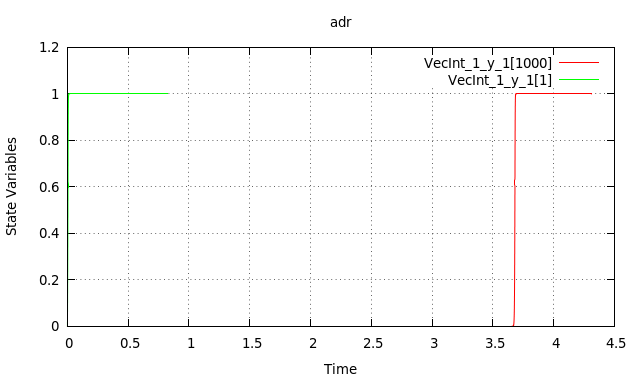
\includegraphics[width=\linewidth]{adr-qss}
\label{graph:adr-qss}
\caption{QSS-Solver}
\end{minipage}
\end{figure}

\section{Convertidor de Voltaje}
	El siguiente modelo es un tipo de convertidor DC - DC que obtiene a su  salida  un  voltaje  continuo  menor  que  a  su entrada, manteniendo una una  alta eficiencia (superior al 95\% con circuitos integrados) y autoregulación.

\begin{align*}
\frac{di_{L}}{dt} & = \frac{-u_{C} - R_D i_D }{L}\\
\frac{du_C}{dt} & =i_D \frac{i_D}{C} - \frac{u_C}{R_L C }
\end{align*}
donde
\begin{align*}
i_D & = \frac{R_s i_L - u_C - U }{R_D + R_s}
\end{align*}


\begin{figure}[H]
\centering
 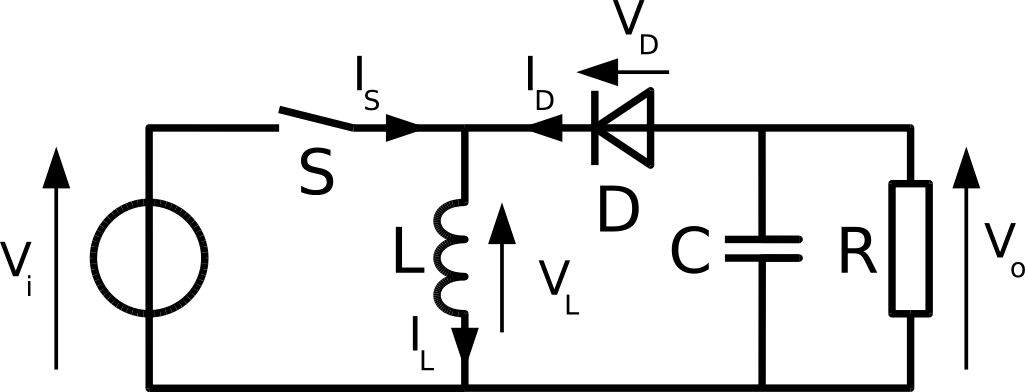
\includegraphics[width=.60\linewidth]{Buckboost_conventions}
 \label{buckdisk-squema}
 \caption{Esquema electrico de convertidor de voltaje}
\end{figure}

\begin{figure}[H]
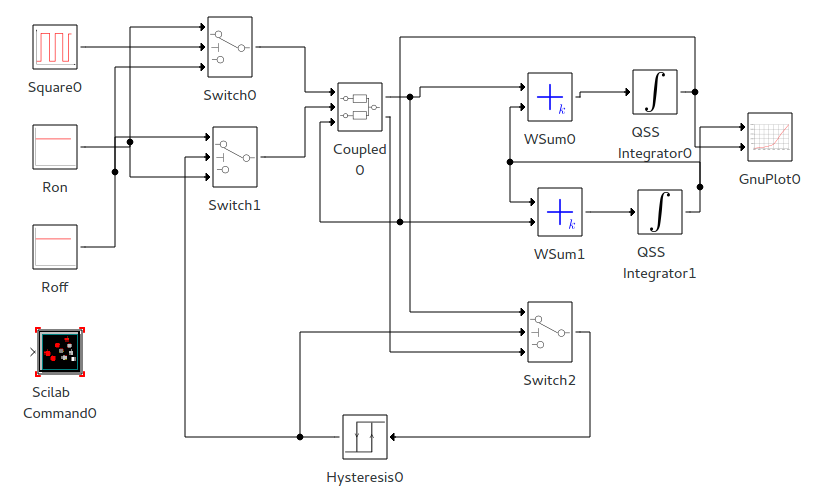
\includegraphics[width=0.75\linewidth]{buck_disk}
 \label{model:buckdisk}
\caption{Modelo Convertidor de voltaje}
\end{figure}

\begin{figure}[H]
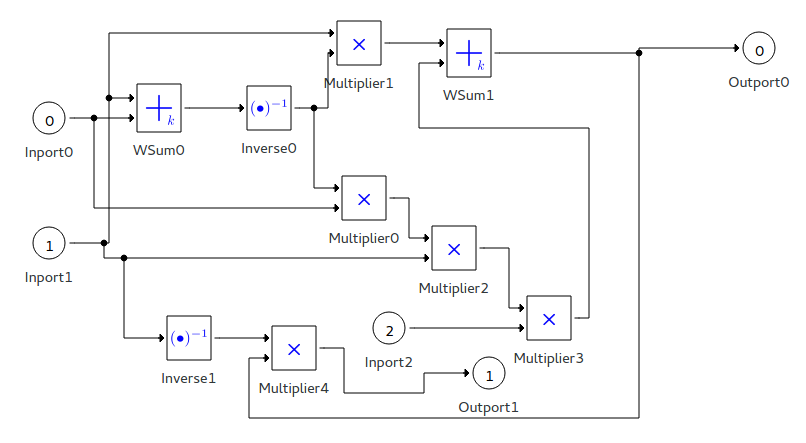
\includegraphics[width=0.75\linewidth]{buck_disk_coupled0}
\caption{Coupled0 (Incluido en Convertidor de voltaje)}
\label{model:buckdisk_coupled0}
\end{figure}

\begin{figure}[H]
\centering
Resultados de la simulación \\
\begin{minipage}{0.5\textwidth}
 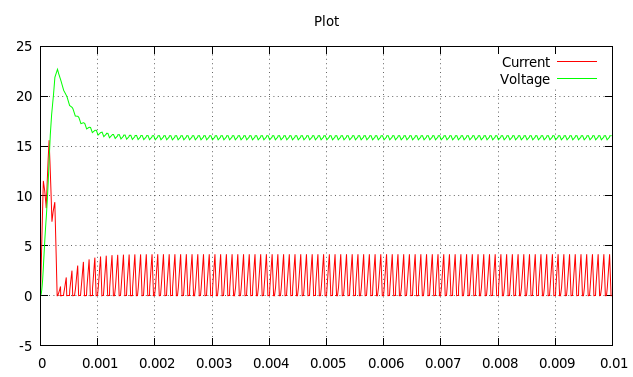
\includegraphics[width=\linewidth]{buck_disk-pd}
\caption{PowerDEVS}
\label{model:buckdisk_coupled0}
\end{minipage}\hfill
\begin{minipage}{0.5\textwidth}
 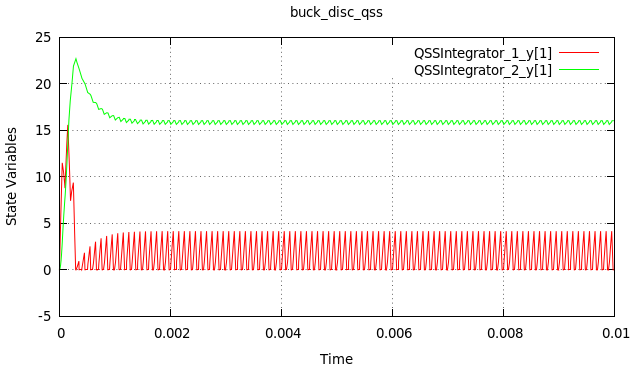
\includegraphics[width=\linewidth]{buck_disk-qss}
\caption{QSS-Solver}
\label{model:buckdisk_coupled0}
\end{minipage}
\end{figure}

\section{Resultados}

\todo[inline]{Qué pruebas? Explicá que vas a hacer una comparación de tiempo de simulación entre los dos enfoques}
	Las pruebas fueron realizadas en una PC Intel\textsuperscript{\textregistered} Core\textsuperscript{TM} i7-3632QM CPU @ 2.20GHz con 16 GB de memoria RAM. Los tiempos observados no deben ser considerados 
	como absolutos ya que variarán de un sistema a otro, pero las mejoras relativas en los tiempos de ejecución deberían mantenerse.

	Los resultados obtenidos son los tiempos observados luego de ejecutar la simulación en PowerDEVS (P.DEVS) y QSS-Solver (QSS-S), ambas mediciones
	son reportadas por los motores de simulación, en milisegundos (ms), todas las simulaciones utilizan el método de integración QSS3 excepto los que 
	se especifica LIQSS2.

\begin{table}[H]
\centering	
\label{my-label}
\begin{tabular}{llllll}
\toprule
{\bf Modelos}            &  {\bf P.DEVS(ms)} & {\bf QSS-S. (ms)} & {\bf Mejora (\%)} \\
\toprule
Lineas de Transmisión 1200s, N=1000     & 76402         & 34982.5         & 54          \\
Inversores(LIQSS2) 250s, N=1000   	& 25046         & 7694.44         & 69        \\
ADR(LIQSS2) 10s, N=1000 		& 6089          & 568.772         & 90        \\
Convertidor de Voltaje 0.01s,        	& 268           & 10.3802         & 96         \\
Lotka  Voltera 300s      		& 11            & 2.75132         & 81

% Mejora esta calculada a partir de 1 - qsssolver / pwdevs
%excepto indicado, se utiliza QSS3
\end{tabular}
\end{table}

	En la tabla se puede ver una mejora entre 54 y 96\% entre todos los modelos, y entre 54 y 90\% para los modelos vectoriales que son nuestro principal objetivo,
	ya que son la forma más simple de realizar grandes modelos, que es lo que esperaba dado que al cambiar de formalismo se evita todo los mensajes entre modelos 
	característico del formalismo DEVS, además de aprobechar la velocidad del QSS-Solver.
